\documentclass[11pt]{article}

\usepackage[margin=1in]{geometry}
\usepackage{graphicx}
\usepackage{array}
\usepackage{longtable}
\usepackage{hyperref}
\usepackage{booktabs}
\usepackage{xcolor}
\usepackage{tikz}
\usepackage{float}
\usepackage{enumitem}
\usepackage{fancyhdr}
\usepackage{titlesec}
\usepackage{tcolorbox}
\usepackage{tabularx}
\usepackage{multirow}
\usepackage{caption}
\usepackage{subcaption}
\usepackage{listings}
\usepackage{makecell}
\usepackage{pgfplots}
\usepackage{amssymb}
\pgfplotsset{compat=1.17}

\usetikzlibrary{shapes.geometric, arrows.meta, positioning, fit, backgrounds, calc, decorations.pathreplacing, shapes.multipart, matrix, shadows, mindmap, trees}

% Color definitions
\definecolor{decisioncolor}{RGB}{70,130,180}
\definecolor{alternativecolor}{RGB}{60,179,113}
\definecolor{tradeoffcolor}{RGB}{255,165,0}
\definecolor{riskcolor}{RGB}{220,53,69}
\definecolor{flowcolor}{RGB}{100,100,100}
\definecolor{sectionblue}{RGB}{31,78,121}
\definecolor{lightgray}{RGB}{245,245,245}
\definecolor{warningred}{RGB}{220,53,69}
\definecolor{successgreen}{RGB}{40,167,69}
\definecolor{infoblue}{RGB}{23,162,184}
\definecolor{drivercolor}{RGB}{186,85,211}
\definecolor{consequencecolor}{RGB}{255,193,7}
\definecolor{acceptedcolor}{RGB}{40,167,69}
\definecolor{rejectedcolor}{RGB}{220,53,69}
\definecolor{deprecatedcolor}{RGB}{108,117,125}
\definecolor{proposedcolor}{RGB}{23,162,184}

% Hyperref setup
\hypersetup{
    colorlinks=true,
    linkcolor=sectionblue,
    urlcolor=sectionblue,
    citecolor=sectionblue
}

% Header and footer
\pagestyle{fancy}
\fancyhf{}
\fancyhead[L]{\leftmark}
\fancyhead[R]{Architectural Rationale Documentation}
\fancyfoot[C]{\thepage}
\renewcommand{\headrulewidth}{0.4pt}
\renewcommand{\footrulewidth}{0.4pt}

% Section formatting
\titleformat{\section}
  {\normalfont\Large\bfseries\color{sectionblue}}{\thesection}{1em}{}
\titleformat{\subsection}
  {\normalfont\large\bfseries\color{sectionblue!80}}{\thesubsection}{1em}{}
\titleformat{\subsubsection}
  {\normalfont\normalsize\bfseries\color{sectionblue!60}}{\thesubsubsection}{1em}{}

% Custom box environments
\newtcolorbox{keypoint}{
    colback=blue!5,
    colframe=sectionblue,
    title=Key Point,
    fonttitle=\bfseries
}

\newtcolorbox{warning}{
    colback=red!5,
    colframe=warningred,
    title=Warning,
    fonttitle=\bfseries
}

\newtcolorbox{bestpractice}{
    colback=green!5,
    colframe=successgreen,
    title=Best Practice,
    fonttitle=\bfseries
}

\newtcolorbox{example}{
    colback=lightgray,
    colframe=flowcolor,
    title=Example,
    fonttitle=\bfseries
}

\newtcolorbox{definition}{
    colback=infoblue!10,
    colframe=infoblue,
    title=Definition,
    fonttitle=\bfseries
}

\newtcolorbox{template}{
    colback=white,
    colframe=flowcolor,
    title=Template,
    fonttitle=\bfseries
}

\newtcolorbox{decisionbox}[1][]{
    colback=decisioncolor!10,
    colframe=decisioncolor,
    title=#1,
    fonttitle=\bfseries
}

\newtcolorbox{adrbox}[1][]{
    colback=lightgray,
    colframe=sectionblue,
    title=#1,
    fonttitle=\bfseries,
    breakable
}

% Code listing style
\lstset{
    basicstyle=\ttfamily\small,
    breaklines=true,
    frame=single,
    backgroundcolor=\color{lightgray},
    keywordstyle=\color{sectionblue},
    commentstyle=\color{successgreen},
    stringstyle=\color{tradeoffcolor}
}

% Custom column types
\newcolumntype{L}[1]{>{\raggedright\arraybackslash}p{#1}}
\newcolumntype{C}[1]{>{\centering\arraybackslash}p{#1}}
\newcolumntype{R}[1]{>{\raggedleft\arraybackslash}p{#1}}

% Status badges
\newcommand{\statusaccepted}{\textcolor{acceptedcolor}{\textbf{[ACCEPTED]}}}
\newcommand{\statusrejected}{\textcolor{rejectedcolor}{\textbf{[REJECTED]}}}
\newcommand{\statusdeprecated}{\textcolor{deprecatedcolor}{\textbf{[DEPRECATED]}}}
\newcommand{\statusproposed}{\textcolor{proposedcolor}{\textbf{[PROPOSED]}}}
\newcommand{\statussuperseded}{\textcolor{tradeoffcolor}{\textbf{[SUPERSEDED]}}}

\title{%
    \vspace{-1cm}
    \textbf{\Huge Software Architecture Documentation}\\[12pt]
    \Large Architectural Rationale\\[8pt]
    \large A Comprehensive Guide to Documenting Design Decisions,\\
    Tradeoffs, Alternatives, and Technical Debt
}
\author{%
    \textit{Architecture Documentation Series}\\[4pt]
    \small Based on ADR Standards, SEI Decision Documentation, and Industry Best Practices
}
\date{\today}

\begin{document}

\maketitle
\thispagestyle{empty}

\vspace{0.8cm}

\begin{abstract}
\noindent
Architectural rationale captures the reasoning behind design decisions---the ``why'' that explains the ``what'' shown in architectural views. Without documented rationale, architectures become inscrutable over time, leading to poor decisions, unnecessary rework, and loss of institutional knowledge. This comprehensive guide establishes principles and practices for documenting architectural rationale, including design drivers, decision records, alternatives analysis, tradeoff evaluation, pattern selection, risk assessment, and technical debt management. The document introduces the Architecture Decision Record (ADR) format, provides frameworks for systematic tradeoff analysis, and establishes governance processes for maintaining rationale documentation throughout the system lifecycle. Whether facing technology choices, structural decisions, or quality attribute tradeoffs, this guide provides the foundation for making decisions transparent, traceable, and defensible.
\end{abstract}

\vfill

\begin{center}
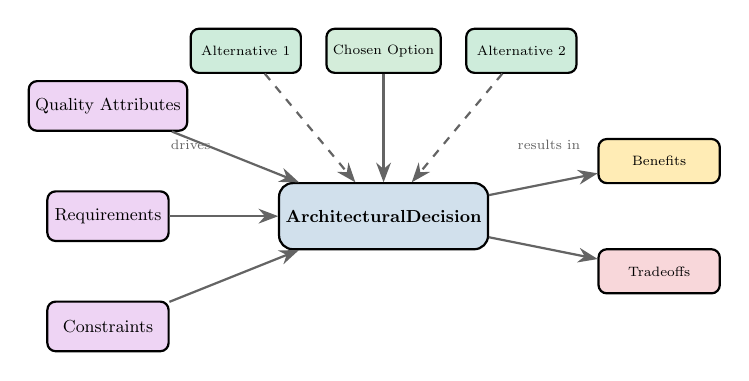
\begin{tikzpicture}[
    scale=0.7,
    transform shape,
    decision/.style={draw, thick, fill=decisioncolor!25, minimum width=3cm, minimum height=1.2cm, rounded corners=5pt, font=\small\bfseries},
    driver/.style={draw, thick, fill=drivercolor!25, minimum width=2.2cm, minimum height=0.9cm, rounded corners=3pt, font=\small},
    alt/.style={draw, thick, fill=alternativecolor!25, minimum width=2cm, minimum height=0.8cm, rounded corners=3pt, font=\scriptsize},
    consequence/.style={draw, thick, fill=consequencecolor!30, minimum width=2.2cm, minimum height=0.8cm, rounded corners=3pt, font=\scriptsize},
    arrow/.style={-{Stealth[length=2.5mm]}, thick, flowcolor}
]
    % Central decision
    \node[decision] (dec) at (0,0) {Architectural\\Decision};
    
    % Drivers (inputs)
    \node[driver] (qa) at (-5,2) {Quality Attributes};
    \node[driver] (req) at (-5,0) {Requirements};
    \node[driver] (con) at (-5,-2) {Constraints};
    
    % Alternatives
    \node[alt, fill=acceptedcolor!20] (chosen) at (0,3) {Chosen Option};
    \node[alt] (alt1) at (-2.5,3) {Alternative 1};
    \node[alt] (alt2) at (2.5,3) {Alternative 2};
    
    % Consequences
    \node[consequence] (pos) at (5,1) {Benefits};
    \node[consequence, fill=riskcolor!20] (neg) at (5,-1) {Tradeoffs};
    
    % Arrows
    \draw[arrow] (qa) -- (dec);
    \draw[arrow] (req) -- (dec);
    \draw[arrow] (con) -- (dec);
    
    \draw[arrow, dashed] (alt1) -- (dec);
    \draw[arrow] (chosen) -- (dec);
    \draw[arrow, dashed] (alt2) -- (dec);
    
    \draw[arrow] (dec) -- (pos);
    \draw[arrow] (dec) -- (neg);
    
    % Labels
    \node[font=\scriptsize, flowcolor] at (-3.5,1.3) {drives};
    \node[font=\scriptsize, flowcolor] at (3,1.3) {results in};
\end{tikzpicture}
\end{center}

\newpage
\tableofcontents
\newpage

%==============================================================================
\section{Introduction to Architectural Rationale}
%==============================================================================

\subsection{Definition and Purpose}

Architectural rationale is the explicit documentation of the reasoning behind architectural decisions. It captures not just what was decided, but why it was decided, what alternatives were considered, what tradeoffs were made, and what consequences are expected.

\begin{definition}
\textbf{Architectural Rationale} is the documentation that explains the reasoning, assumptions, tradeoffs, and constraints that led to the architectural decisions reflected in a system's design. It answers the question ``why is the architecture this way?'' and preserves the decision-making context for future reference.
\end{definition}

Documenting rationale serves several critical purposes. First, it provides \textbf{knowledge preservation} by capturing the reasoning that would otherwise exist only in the minds of original architects. Second, it enables \textbf{informed evolution} by allowing future architects to understand constraints and tradeoffs before making changes. Third, it ensures \textbf{decision quality} by forcing explicit consideration of alternatives and consequences. Fourth, it supports \textbf{stakeholder communication} by explaining architectural choices to diverse audiences. Fifth, it creates \textbf{accountability} through transparent, traceable decision-making. Sixth, it prevents \textbf{decision erosion} by documenting why certain approaches were rejected.

\subsection{The Cost of Missing Rationale}

Organizations that fail to document rationale pay significant costs over time.

\begin{warning}
\textbf{Consequences of Undocumented Rationale:}

\textbf{Repeated Mistakes:} Teams revisit rejected alternatives because they don't know why they were rejected, wasting time rediscovering the same problems.

\textbf{Inappropriate Changes:} Modifications that violate implicit constraints break the system in subtle ways because the constraints were never documented.

\textbf{Knowledge Loss:} When original architects leave, critical understanding leaves with them, creating ``legacy'' systems that no one fully understands.

\textbf{Analysis Paralysis:} Without documented precedents, teams struggle to make decisions, fearing unknown consequences.

\textbf{Inconsistent Decisions:} Similar problems are solved differently across the system because there's no record of previous approaches.
\end{warning}

\subsection{Rationale Within Architectural Documentation}

Rationale documentation complements the structural documentation in architectural views. While primary presentations and element catalogs describe what the architecture is, rationale explains why it is that way.

\begin{figure}[H]
\centering
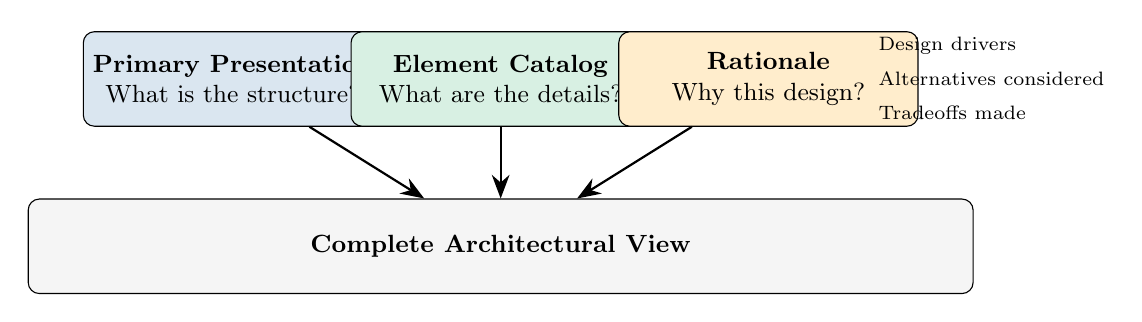
\begin{tikzpicture}[
    scale=0.85,
    box/.style={draw, rounded corners, minimum width=3.8cm, minimum height=1.2cm, align=center, font=\small},
    arrow/.style={-{Stealth[length=3mm]}, thick}
]
    % View components
    \node[box, fill=decisioncolor!20] (primary) at (-4,2) {\textbf{Primary Presentation}\\What is the structure?};
    \node[box, fill=alternativecolor!20] (catalog) at (0,2) {\textbf{Element Catalog}\\What are the details?};
    \node[box, fill=tradeoffcolor!20] (rationale) at (4,2) {\textbf{Rationale}\\Why this design?};
    
    % Complete view
    \node[box, fill=lightgray, minimum width=12cm] (view) at (0,-0.5) {\textbf{Complete Architectural View}};
    
    % Arrows
    \draw[arrow] (primary) -- (view);
    \draw[arrow] (catalog) -- (view);
    \draw[arrow] (rationale) -- (view);
    
    % Questions answered
    \node[font=\scriptsize, right] at (5.5,2.5) {Design drivers};
    \node[font=\scriptsize, right] at (5.5,2) {Alternatives considered};
    \node[font=\scriptsize, right] at (5.5,1.5) {Tradeoffs made};
\end{tikzpicture}
\caption{Rationale as Part of Complete Architectural Documentation}
\end{figure}

\subsection{Standards and Frameworks}

Architectural rationale documentation draws from several established approaches. The SEI (Software Engineering Institute) views and beyond approach includes rationale as part of every architectural view. Architecture Decision Records (ADRs) provide a lightweight format popularized by Michael Nygard for capturing decisions. ISO/IEC/IEEE 42010 establishes requirements for architecture rationale in architecture descriptions. Design Rationale Systems from academic research provide formal models for capturing design reasoning. TOGAF includes architecture decision documentation as part of the Architecture Development Method.

%==============================================================================
\section{Design Drivers}
%==============================================================================

\subsection{Understanding Design Drivers}

Design drivers are the forces that shape architectural decisions. They include functional requirements, quality attribute requirements, constraints, and business goals. Understanding and documenting drivers is essential because they provide the ``why'' behind decisions.

\begin{figure}[H]
\centering
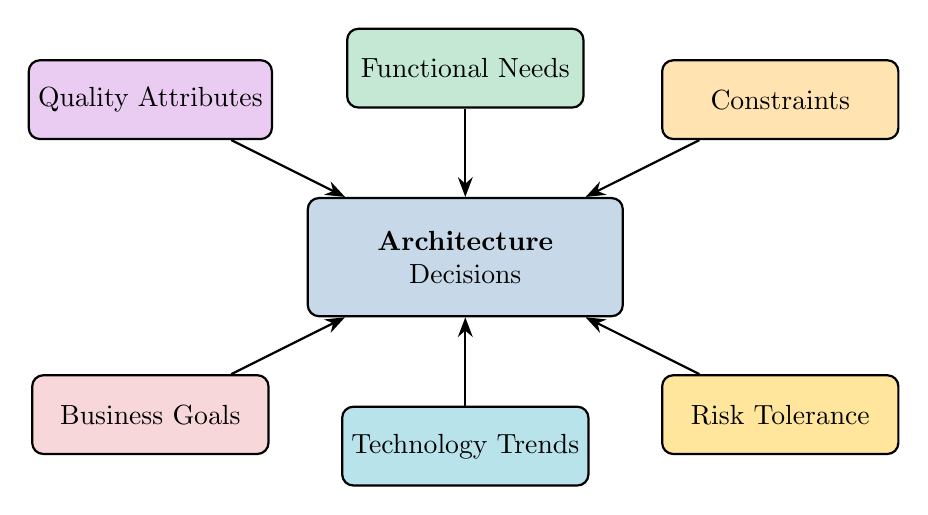
\begin{tikzpicture}[
    scale=0.8,
    driver/.style={draw, thick, rounded corners, minimum width=3cm, minimum height=1cm, align=center},
    arrow/.style={-{Stealth[length=2.5mm]}, thick}
]
    % Central architecture
    \node[driver, fill=decisioncolor!30, minimum width=4cm, minimum height=1.5cm] (arch) at (0,0) {\textbf{Architecture}\\Decisions};
    
    % Driver categories
    \node[driver, fill=drivercolor!30] (qa) at (-5,2.5) {Quality Attributes};
    \node[driver, fill=alternativecolor!30] (func) at (0,3) {Functional Needs};
    \node[driver, fill=tradeoffcolor!30] (const) at (5,2.5) {Constraints};
    \node[driver, fill=riskcolor!20] (bus) at (-5,-2.5) {Business Goals};
    \node[driver, fill=infoblue!30] (tech) at (0,-3) {Technology Trends};
    \node[driver, fill=consequencecolor!40] (risk) at (5,-2.5) {Risk Tolerance};
    
    % Arrows
    \draw[arrow] (qa) -- (arch);
    \draw[arrow] (func) -- (arch);
    \draw[arrow] (const) -- (arch);
    \draw[arrow] (bus) -- (arch);
    \draw[arrow] (tech) -- (arch);
    \draw[arrow] (risk) -- (arch);
\end{tikzpicture}
\caption{Categories of Design Drivers}
\end{figure}

\subsection{Quality Attribute Drivers}

Quality attributes (non-functional requirements) are among the most important drivers of architectural decisions. Structure exists largely to achieve quality attributes.

\subsubsection{Quality Attribute Scenarios}

Document quality attribute drivers as concrete, testable scenarios using the SEI quality attribute scenario format.

\begin{template}
\textbf{Quality Attribute Scenario Template}

\vspace{0.2cm}
\begin{tabular}{@{}L{3cm} L{9.5cm}@{}}
\textbf{Scenario ID:} & Unique identifier (e.g., QA-PERF-001) \\
\textbf{Quality Attribute:} & The quality attribute addressed (e.g., Performance) \\
\textbf{Source:} & Entity that generates the stimulus \\
\textbf{Stimulus:} & The event or condition that affects the system \\
\textbf{Environment:} & Conditions under which the stimulus occurs \\
\textbf{Artifact:} & Part of system that is stimulated \\
\textbf{Response:} & How the system should respond \\
\textbf{Response Measure:} & Quantifiable measure of the response \\
\end{tabular}
\end{template}

\begin{example}
\textbf{Quality Attribute Scenario: QA-PERF-001}

\vspace{0.2cm}
\begin{tabular}{@{}L{3cm} L{9.5cm}@{}}
\textbf{Quality Attribute:} & Performance (Latency) \\
\textbf{Source:} & External customer \\
\textbf{Stimulus:} & Submits order during peak shopping period \\
\textbf{Environment:} & Normal operation, Black Friday traffic (10x normal) \\
\textbf{Artifact:} & Order processing system \\
\textbf{Response:} & Order is validated, inventory reserved, confirmation returned \\
\textbf{Response Measure:} & 95th percentile response time $\leq$ 2 seconds \\
\end{tabular}

\vspace{0.2cm}
\textbf{Architectural Impact:} This scenario drives decisions toward horizontal scaling, caching, and asynchronous processing for non-critical path operations.
\end{example}

\subsubsection{Quality Attribute Priority Matrix}

Not all quality attributes are equally important. Document relative priorities to guide tradeoff decisions.

\begin{longtable}{@{}L{2.5cm} C{1.5cm} L{4cm} L{4.5cm}@{}}
\caption{Quality Attribute Priority Matrix} \\
\toprule
\textbf{Attribute} & \textbf{Priority} & \textbf{Key Scenarios} & \textbf{Architectural Impact} \\
\midrule
\endfirsthead
\toprule
\textbf{Attribute} & \textbf{Priority} & \textbf{Key Scenarios} & \textbf{Architectural Impact} \\
\midrule
\endhead
\bottomrule
\endlastfoot
Availability & Critical & 99.95\% uptime; graceful degradation & Redundancy; health checks; failover \\
Performance & High & 2s response at 10x load & Caching; async processing; CDN \\
Security & High & PCI compliance; data protection & Encryption; auth/authz; audit logging \\
Scalability & High & Handle 100K concurrent users & Stateless services; horizontal scaling \\
Modifiability & Medium & Deploy changes within 1 day & Microservices; CI/CD; feature flags \\
Testability & Medium & 80\% code coverage; automated testing & Dependency injection; interfaces \\
Usability & Medium & Task completion within 3 clicks & API design; error messages \\
Cost & Medium & Operate within \$50K/month & Cloud optimization; reserved instances \\
\end{longtable}

\subsection{Constraints}

Constraints are non-negotiable requirements that limit architectural options. Unlike quality attributes (which involve tradeoffs), constraints are absolute.

\subsubsection{Constraint Categories}

\begin{longtable}{@{}L{3cm} L{4cm} L{5.5cm}@{}}
\caption{Constraint Categories and Examples} \\
\toprule
\textbf{Category} & \textbf{Examples} & \textbf{Typical Sources} \\
\midrule
\endfirsthead
\toprule
\textbf{Category} & \textbf{Examples} & \textbf{Typical Sources} \\
\midrule
\endhead
\bottomrule
\endlastfoot
Technical & Must use Java; must deploy to AWS; must integrate with SAP & Enterprise standards; existing investments \\
Organizational & Maximum team size of 8; must be maintainable by existing staff & HR policies; skill availability \\
Regulatory & PCI-DSS compliance; GDPR data residency; SOX audit requirements & Government; industry bodies \\
Contractual & Must use vendor X for payments; SLA commitments to customers & Business agreements; partnerships \\
Financial & Development budget of \$500K; operational budget of \$5K/month & Business planning; funding \\
Schedule & Must launch by Q4; integration complete by March & Market timing; dependencies \\
Physical & Must operate in edge locations with limited connectivity & Deployment environment \\
\end{longtable}

\subsubsection{Constraint Documentation}

\begin{longtable}{@{}L{1.2cm} L{3.5cm} L{2.5cm} L{2.5cm} L{2.5cm}@{}}
\caption{Constraint Registry} \\
\toprule
\textbf{ID} & \textbf{Constraint} & \textbf{Category} & \textbf{Source} & \textbf{Impact} \\
\midrule
\endfirsthead
\toprule
\textbf{ID} & \textbf{Constraint} & \textbf{Category} & \textbf{Source} & \textbf{Impact} \\
\midrule
\endhead
\bottomrule
\endlastfoot
CON-01 & Must deploy to AWS only & Technical & Enterprise IT policy & Eliminates multi-cloud options \\
CON-02 & Java or Kotlin for backend services & Technical & Team skills; hiring & Limits technology choices \\
CON-03 & PCI-DSS Level 1 compliance & Regulatory & Payment processing & Isolation; encryption; audit \\
CON-04 & EU data must stay in EU & Regulatory & GDPR & Multi-region deployment \\
CON-05 & Budget: \$50K/month operations & Financial & Business case & Cloud cost optimization \\
CON-06 & Launch by November 1 & Schedule & Holiday season & Phased delivery; MVP scope \\
\end{longtable}

\subsection{Key Requirements}

Certain functional requirements significantly influence architecture. These architecturally significant requirements (ASRs) should be explicitly identified.

\begin{keypoint}
\textbf{Identifying Architecturally Significant Requirements:}

A requirement is architecturally significant if it:
\begin{itemize}[nosep]
    \item Has broad effect on the system structure
    \item Affects a quality attribute to a significant degree
    \item Involves tradeoffs between quality attributes
    \item Requires unusual or innovative solutions
    \item Has high business or technical risk
    \item Constrains future evolution
\end{itemize}
\end{keypoint}

\begin{longtable}{@{}L{1.2cm} L{4.5cm} L{3cm} L{3.5cm}@{}}
\caption{Architecturally Significant Requirements} \\
\toprule
\textbf{ID} & \textbf{Requirement} & \textbf{Category} & \textbf{Architectural Impact} \\
\midrule
\endfirsthead
\toprule
\textbf{ID} & \textbf{Requirement} & \textbf{Category} & \textbf{Architectural Impact} \\
\midrule
\endhead
\bottomrule
\endlastfoot
ASR-01 & Process 10,000 orders per minute at peak & Performance & Horizontal scaling; async processing \\
ASR-02 & Support real-time inventory across 500 stores & Integration & Event-driven; eventual consistency \\
ASR-03 & Enable A/B testing of all features & Modifiability & Feature flags; canary deployment \\
ASR-04 & Maintain audit trail for 7 years & Compliance & Event sourcing; archival storage \\
ASR-05 & Support offline operation for mobile POS & Availability & Local storage; sync protocol \\
\end{longtable}

%==============================================================================
\section{Architecture Decision Records (ADRs)}
%==============================================================================

\subsection{Introduction to ADRs}

Architecture Decision Records (ADRs) are a lightweight format for capturing architectural decisions. Popularized by Michael Nygard, ADRs provide a standardized, version-controlled approach to decision documentation.

\begin{definition}
An \textbf{Architecture Decision Record (ADR)} is a document that captures a single architectural decision along with its context, considered alternatives, rationale, and consequences. ADRs are typically stored alongside code in version control, making decision history part of the project repository.
\end{definition}

\subsection{ADR Format}

The standard ADR format includes several key sections.

\begin{template}
\textbf{Architecture Decision Record Template}

\vspace{0.3cm}
\textbf{Title:} ADR-NNN: Short Descriptive Title

\vspace{0.2cm}
\textbf{Status:} [Proposed | Accepted | Deprecated | Superseded by ADR-XXX]

\vspace{0.2cm}
\textbf{Date:} YYYY-MM-DD

\vspace{0.2cm}
\textbf{Context:}\\
Describe the forces at play, including technological, political, social, and project constraints. This section should be value-neutral---simply describe the facts.

\vspace{0.2cm}
\textbf{Decision:}\\
State the decision in full sentences, with an active voice. ``We will...''

\vspace{0.2cm}
\textbf{Consequences:}\\
Describe the resulting context after applying the decision. All consequences should be listed, both positive and negative. A decision that appears to have only positive consequences is likely missing something.

\vspace{0.2cm}
\textbf{Alternatives Considered:}\\
List alternatives that were evaluated and why they were not chosen.
\end{template}

\subsection{ADR Lifecycle}

ADRs have a lifecycle that reflects the evolution of architectural decisions.

\begin{figure}[H]
\centering
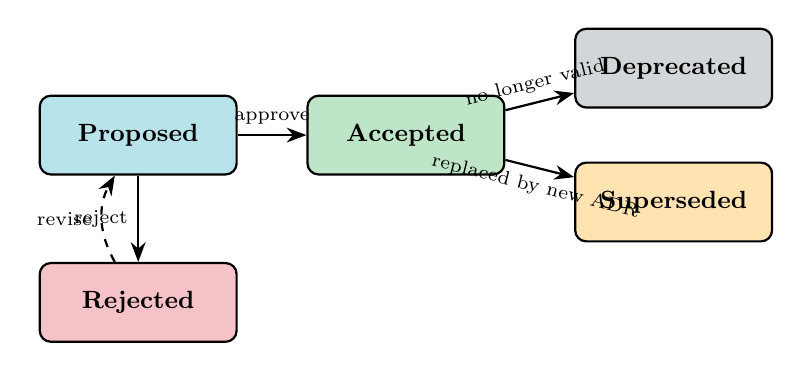
\begin{tikzpicture}[
    scale=0.85,
    state/.style={draw, thick, rounded corners, minimum width=2.5cm, minimum height=1cm, font=\small\bfseries},
    trans/.style={-{Stealth[length=2.5mm]}, thick}
]
    % States
    \node[state, fill=proposedcolor!30] (proposed) at (0,0) {Proposed};
    \node[state, fill=acceptedcolor!30] (accepted) at (4,0) {Accepted};
    \node[state, fill=deprecatedcolor!30] (deprecated) at (8,1) {Deprecated};
    \node[state, fill=tradeoffcolor!30] (superseded) at (8,-1) {Superseded};
    \node[state, fill=rejectedcolor!30] (rejected) at (0,-2.5) {Rejected};
    
    % Transitions
    \draw[trans] (proposed) -- node[above, font=\scriptsize] {approve} (accepted);
    \draw[trans] (proposed) -- node[left, font=\scriptsize] {reject} (rejected);
    \draw[trans] (accepted) -- node[above, font=\scriptsize, sloped] {no longer valid} (deprecated);
    \draw[trans] (accepted) -- node[below, font=\scriptsize, sloped] {replaced by new ADR} (superseded);
    
    % Loop back
    \draw[trans, dashed] (rejected) to[bend left=30] node[left, font=\scriptsize] {revise} (proposed);
\end{tikzpicture}
\caption{ADR Lifecycle States}
\end{figure}

\subsubsection{ADR Status Definitions}

\begin{longtable}{@{}L{2.5cm} L{10cm}@{}}
\caption{ADR Status Definitions} \\
\toprule
\textbf{Status} & \textbf{Description} \\
\midrule
\endfirsthead
\toprule
\textbf{Status} & \textbf{Description} \\
\midrule
\endhead
\bottomrule
\endlastfoot
\statusproposed & Decision is proposed but not yet approved. Open for discussion. \\
\statusaccepted & Decision has been approved and is in effect. Implementation should follow. \\
\statusrejected & Decision was considered but rejected. Rationale preserved for future reference. \\
\statusdeprecated & Decision is no longer recommended but may still be in use. Plan for migration. \\
\statussuperseded & Decision has been replaced by a newer decision. Link to replacement ADR. \\
\end{longtable}

\subsection{Complete ADR Examples}

\begin{adrbox}[ADR-001: Use PostgreSQL for Primary Data Storage]

\textbf{Status:} \statusaccepted

\textbf{Date:} 2024-01-15

\textbf{Deciders:} Architecture Team, Database Team Lead

\vspace{0.3cm}
\textbf{Context}

We need to select a primary database for the e-commerce platform. The database will store orders, customers, products, and inventory data. Key requirements include:
\begin{itemize}[nosep]
    \item ACID transactions for order processing
    \item Complex queries for reporting and analytics
    \item Support for JSON documents for flexible product attributes
    \item Mature ecosystem with strong operational tooling
    \item Team familiarity and hiring availability
\end{itemize}

Current transaction volume is approximately 1,000 orders/hour with projected growth to 10,000 orders/hour within 2 years. Data volume is estimated at 500GB initially, growing to 5TB over 3 years.

\vspace{0.3cm}
\textbf{Decision}

We will use PostgreSQL 15 as our primary relational database.

\vspace{0.3cm}
\textbf{Consequences}

\textit{Positive:}
\begin{itemize}[nosep]
    \item Strong ACID compliance ensures data integrity for financial transactions
    \item Excellent JSON/JSONB support provides flexibility without sacrificing relational model
    \item Mature replication and backup solutions (streaming replication, pgBackRest)
    \item Strong community and commercial support options
    \item Team has existing PostgreSQL expertise
    \item Available as managed service on AWS (RDS, Aurora PostgreSQL)
\end{itemize}

\textit{Negative:}
\begin{itemize}[nosep]
    \item Horizontal scaling is more complex than NoSQL alternatives
    \item May need read replicas for high-read workloads
    \item Requires careful schema design and indexing for performance
    \item Not optimal for time-series data (will need separate solution)
\end{itemize}

\textit{Risks:}
\begin{itemize}[nosep]
    \item If transaction volume exceeds projections significantly, may need sharding strategy
    \item Schema migrations require careful planning for zero-downtime deployments
\end{itemize}

\vspace{0.3cm}
\textbf{Alternatives Considered}

\textbf{MySQL/MariaDB:} Similar capabilities but team has less experience. PostgreSQL's JSONB support is superior.

\textbf{MongoDB:} Better horizontal scaling but weaker transaction support. ACID transactions added recently but less mature. Would complicate joins for reporting.

\textbf{Amazon DynamoDB:} Excellent scaling but requires significant application changes for query patterns. Complex for ad-hoc reporting. Higher cost at our data volumes.

\textbf{CockroachDB:} Better horizontal scaling than PostgreSQL but less mature, smaller talent pool, and higher operational complexity.
\end{adrbox}

\begin{adrbox}[ADR-002: Adopt Event-Driven Architecture for Service Communication]

\textbf{Status:} \statusaccepted

\textbf{Date:} 2024-01-22

\textbf{Deciders:} Architecture Team, Platform Team Lead

\vspace{0.3cm}
\textbf{Context}

Our microservices architecture requires inter-service communication. Currently considering two primary patterns:
\begin{itemize}[nosep]
    \item Synchronous: Direct HTTP/gRPC calls between services
    \item Asynchronous: Event-driven communication via message broker
\end{itemize}

Key considerations include:
\begin{itemize}[nosep]
    \item Resilience to service failures
    \item Ability to handle traffic spikes
    \item Maintaining data consistency across services
    \item Supporting audit requirements (7-year retention)
    \item Team familiarity with patterns
\end{itemize}

The Order Service must coordinate with Inventory, Payment, and Notification services. Order completion rate must remain above 99.9\% even during partial outages.

\vspace{0.3cm}
\textbf{Decision}

We will adopt an event-driven architecture using Apache Kafka as the primary message broker for inter-service communication. Synchronous calls will be limited to:
\begin{itemize}[nosep]
    \item User-facing APIs requiring immediate response
    \item Queries that cannot tolerate eventual consistency
\end{itemize}

\vspace{0.3cm}
\textbf{Consequences}

\textit{Positive:}
\begin{itemize}[nosep]
    \item Services are decoupled; failures don't cascade
    \item Natural buffering handles traffic spikes
    \item Event log provides audit trail and enables replay
    \item Supports multiple consumers without sender changes
    \item Easier to add new services (subscribe to existing events)
\end{itemize}

\textit{Negative:}
\begin{itemize}[nosep]
    \item Eventual consistency requires careful design
    \item Debugging distributed workflows is more complex
    \item Additional infrastructure (Kafka cluster) to operate
    \item Team needs training on event-driven patterns
    \item Message schema evolution requires governance
\end{itemize}

\textit{Risks:}
\begin{itemize}[nosep]
    \item Consumer lag could cause stale data if not monitored
    \item Poison messages could block processing without dead-letter handling
\end{itemize}

\vspace{0.3cm}
\textbf{Alternatives Considered}

\textbf{Pure Synchronous (REST/gRPC):} Simpler mental model but creates tight coupling. Single service failure can cascade. Difficult to handle spikes without circuit breakers everywhere.

\textbf{RabbitMQ:} Simpler than Kafka but lacks event replay capability. Our audit requirements benefit from Kafka's log retention.

\textbf{AWS SQS/SNS:} Easier to operate but less control over partitioning. Kafka's consumer groups provide better scaling model for our use case.
\end{adrbox}

\subsection{ADR Organization and Naming}

\begin{bestpractice}
\textbf{ADR Organization Guidelines:}

\textbf{Location:} Store ADRs in version control alongside code, typically in \texttt{docs/adr/} or \texttt{architecture/decisions/}.

\textbf{Naming:} Use sequential numbering with descriptive titles:
\begin{itemize}[nosep]
    \item \texttt{0001-use-postgresql-for-primary-storage.md}
    \item \texttt{0002-adopt-event-driven-architecture.md}
    \item \texttt{0003-select-kubernetes-for-orchestration.md}
\end{itemize}

\textbf{Format:} Markdown is most common for compatibility with GitHub/GitLab rendering.

\textbf{Index:} Maintain an index file (README.md) linking to all ADRs with status.

\textbf{Immutability:} Once accepted, ADRs should not be modified except to update status. Create new ADRs to supersede old ones.
\end{bestpractice}

\subsection{Decision Log Summary}

Maintain a summary table for quick reference to all decisions.

\setlength{\extrarowheight}{4pt}
\begin{longtable}{@{}L{1.3cm} L{3.5cm} L{1.8cm} L{2.5cm} L{3cm}@{}}
\caption{Architecture Decision Log} \\
\toprule
\textbf{ID} & \textbf{Decision} & \textbf{Status} & \textbf{Date} & \textbf{Key Drivers} \\
\midrule
\endfirsthead
\toprule
\textbf{ID} & \textbf{Decision} & \textbf{Status} & \textbf{Date} & \textbf{Key Drivers} \\
\midrule
\endhead
\midrule
\multicolumn{5}{r}{\textit{Continued on next page}} \\
\endfoot
\bottomrule
\endlastfoot
ADR-001 & PostgreSQL for primary DB & \statusaccepted & 2024-01-15 & ACID; team skills \\
ADR-002 & Event-driven architecture & \statusaccepted & 2024-01-22 & Resilience; audit \\
ADR-003 & Kubernetes for orchestration & \statusaccepted & 2024-02-01 & Scaling; portability \\
ADR-004 & JWT for authentication & \statusaccepted & 2024-02-08 & Stateless; standards \\
ADR-005 & GraphQL for mobile API & \statusproposed & 2024-02-15 & Bandwidth; flexibility \\
ADR-006 & Session-based auth & \statussuperseded & 2024-01-10 & Superseded by ADR-004 \\
\end{longtable}

%==============================================================================
\section{Alternatives Analysis}
%==============================================================================

\subsection{Systematic Alternatives Evaluation}

Thorough evaluation of alternatives is essential for sound decision-making. A systematic approach ensures consistency and completeness.

\subsubsection{Alternatives Identification}

Before evaluating alternatives, ensure you have identified a sufficient range of options.

\begin{bestpractice}
\textbf{Finding Alternatives:}
\begin{itemize}[nosep]
    \item Research industry practices and case studies
    \item Consult technology radar and analyst reports
    \item Review competitor and peer architectures
    \item Brainstorm with diverse team members
    \item Consider ``do nothing'' as a baseline
    \item Include build vs. buy vs. open-source options
    \item Explore hybrid approaches
\end{itemize}
\end{bestpractice}

\subsection{Evaluation Criteria}

Define explicit criteria before evaluating alternatives to ensure objective comparison.

\begin{longtable}{@{}L{3cm} L{5cm} L{4.5cm}@{}}
\caption{Common Evaluation Criteria} \\
\toprule
\textbf{Category} & \textbf{Criteria} & \textbf{Typical Measures} \\
\midrule
\endfirsthead
\toprule
\textbf{Category} & \textbf{Criteria} & \textbf{Typical Measures} \\
\midrule
\endhead
\bottomrule
\endlastfoot
Fitness & Meets functional requirements & Feature coverage percentage \\
Fitness & Meets quality attributes & Scenario satisfaction \\
Cost & Initial development cost & Person-months; \$ \\
Cost & Ongoing operational cost & Monthly \$; person-hours \\
Cost & Licensing cost & Annual \$; per-user \$ \\
Risk & Technical risk & Probability $\times$ impact \\
Risk & Vendor/community viability & Market share; funding \\
Capability & Team skills match & Training required \\
Capability & Tool and ecosystem maturity & Age; adoption; documentation \\
Strategic & Alignment with roadmap & Fit with future plans \\
Strategic & Vendor relationship & Existing contracts; support \\
\end{longtable}

\subsection{Decision Matrix Method}

A decision matrix provides structured comparison of alternatives against weighted criteria.

\begin{example}
\textbf{Database Selection Decision Matrix}

\vspace{0.3cm}
\textbf{Criteria Weights:}
\begin{tabular}{@{}L{4cm} C{2cm}@{}}
ACID Compliance & 25\% \\
Query Flexibility & 20\% \\
Scalability & 20\% \\
Operational Simplicity & 15\% \\
Team Experience & 10\% \\
Cost & 10\% \\
\end{tabular}

\vspace{0.3cm}
\textbf{Scoring (1-5 scale):}

\begin{tabular}{@{}L{3cm} C{1.5cm} C{1.5cm} C{1.5cm} C{1.5cm} C{1.5cm}@{}}
\toprule
\textbf{Criterion} & \textbf{Weight} & \textbf{Postgres} & \textbf{MySQL} & \textbf{MongoDB} & \textbf{DynamoDB} \\
\midrule
ACID Compliance & 25\% & 5 & 4 & 3 & 4 \\
Query Flexibility & 20\% & 5 & 4 & 4 & 2 \\
Scalability & 20\% & 3 & 3 & 5 & 5 \\
Operational Simplicity & 15\% & 4 & 4 & 3 & 5 \\
Team Experience & 10\% & 5 & 3 & 2 & 2 \\
Cost & 10\% & 4 & 4 & 3 & 3 \\
\midrule
\textbf{Weighted Score} & & \textbf{4.25} & \textbf{3.65} & \textbf{3.45} & \textbf{3.65} \\
\bottomrule
\end{tabular}

\vspace{0.3cm}
\textbf{Result:} PostgreSQL scores highest, primarily due to strong ACID compliance, query flexibility, and team experience.
\end{example}

\subsection{Pros and Cons Analysis}

For each alternative, document advantages and disadvantages systematically.

\begin{longtable}{@{}L{2.5cm} L{5cm} L{5cm}@{}}
\caption{Alternative: MongoDB for Primary Storage} \\
\toprule
\textbf{Category} & \textbf{Pros} & \textbf{Cons} \\
\midrule
\endfirsthead
\toprule
\textbf{Category} & \textbf{Pros} & \textbf{Cons} \\
\midrule
\endhead
\bottomrule
\endlastfoot
Functionality & Flexible schema for varying product types; native JSON & Weaker multi-document transactions; joins require application logic \\
Performance & Excellent write throughput; built-in sharding & Index management complexity; query optimization less mature \\
Operations & Easy horizontal scaling; managed service available & Memory-hungry; backup complexity for large datasets \\
Team & Modern developer experience & Limited team experience; training needed \\
Ecosystem & Good driver support; active community & Fewer BI tool integrations \\
Cost & Open source core; pay for Enterprise features & Higher storage costs; Atlas pricing at scale \\
\end{longtable}

\subsection{Sensitivity Analysis}

Test how robust the decision is to changes in criteria weights or scores.

\begin{keypoint}
Perform sensitivity analysis when:
\begin{itemize}[nosep]
    \item The top alternatives are close in score
    \item Criteria weights are uncertain or contested
    \item Future conditions may change criteria importance
    \item Stakeholders have different priorities
\end{itemize}

Ask: ``What would have to change for a different alternative to win?'' If the answer is ``very little,'' the decision may need more deliberation.
\end{keypoint}

%==============================================================================
\section{Tradeoff Analysis}
%==============================================================================

\subsection{Understanding Tradeoffs}

Architecture is fundamentally about tradeoffs. Improving one quality attribute often comes at the expense of another. Documenting tradeoffs explicitly helps stakeholders understand the implications of decisions.

\begin{figure}[H]
\centering
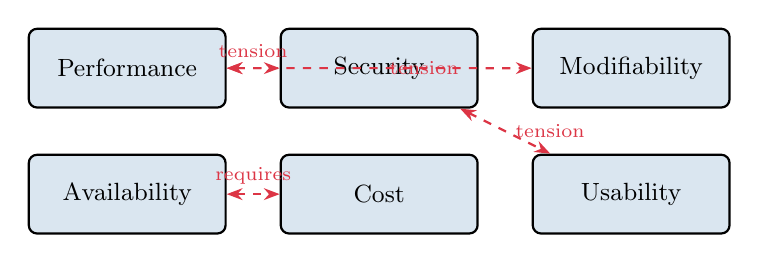
\begin{tikzpicture}[
    scale=0.8,
    attr/.style={draw, thick, fill=decisioncolor!20, minimum width=2.5cm, minimum height=1cm, rounded corners=3pt, font=\small},
    tradeoff/.style={{Stealth[length=2mm]}-{Stealth[length=2mm]}, thick, riskcolor, dashed}
]
    % Quality attributes
    \node[attr] (perf) at (0,2) {Performance};
    \node[attr] (sec) at (4,2) {Security};
    \node[attr] (mod) at (8,2) {Modifiability};
    
    \node[attr] (avail) at (0,0) {Availability};
    \node[attr] (cost) at (4,0) {Cost};
    \node[attr] (usab) at (8,0) {Usability};
    
    % Tradeoff relationships
    \draw[tradeoff] (perf) -- node[above, font=\scriptsize, sloped] {tension} (sec);
    \draw[tradeoff] (perf) -- node[right, font=\scriptsize] {tension} (mod);
    \draw[tradeoff] (avail) -- node[above, font=\scriptsize] {requires} (cost);
    \draw[tradeoff] (sec) -- node[right, font=\scriptsize] {tension} (usab);
\end{tikzpicture}
\caption{Common Quality Attribute Tradeoffs}
\end{figure}

\subsection{Common Tradeoff Patterns}

\begin{longtable}{@{}L{4cm} L{4.5cm} L{4cm}@{}}
\caption{Common Architectural Tradeoffs} \\
\toprule
\textbf{Tradeoff} & \textbf{Description} & \textbf{Mitigation Strategies} \\
\midrule
\endfirsthead
\toprule
\textbf{Tradeoff} & \textbf{Description} & \textbf{Mitigation Strategies} \\
\midrule
\endhead
\bottomrule
\endlastfoot
Performance vs. Security & Encryption and validation add latency & Hardware acceleration; caching; async validation \\
Availability vs. Consistency & CAP theorem; strong consistency limits availability & Eventual consistency where acceptable; careful partition design \\
Modifiability vs. Performance & Abstraction layers add overhead & Profile-driven optimization; bypass for hot paths \\
Simplicity vs. Flexibility & Generic solutions are more complex & Build for current needs; design for extension \\
Time-to-Market vs. Quality & Fast delivery may incur technical debt & MVP scope; planned remediation; feature flags \\
Cost vs. Scalability & Over-provisioning wastes money; under-provisioning limits growth & Auto-scaling; reserved capacity for baseline \\
Usability vs. Security & Security measures can frustrate users & Risk-based authentication; SSO; biometrics \\
\end{longtable}

\subsection{ATAM-Style Tradeoff Documentation}

The Architecture Tradeoff Analysis Method (ATAM) provides a structured approach to analyzing tradeoffs.

\begin{template}
\textbf{Tradeoff Point Documentation}

\vspace{0.2cm}
\textbf{Tradeoff ID:} Unique identifier

\textbf{Decision:} The architectural decision creating the tradeoff

\textbf{Quality Attributes Affected:} List of QAs in tension

\textbf{Description:} Explanation of the tradeoff

\textbf{Sensitivity:} How sensitive is the outcome to this tradeoff?

\textbf{Stakeholder Impact:} Which stakeholders are affected?

\textbf{Mitigation:} How the negative impacts are addressed
\end{template}

\begin{example}
\textbf{Tradeoff Point: TP-001}

\vspace{0.2cm}
\textbf{Decision:} ADR-002 (Event-driven architecture)

\textbf{Quality Attributes:} Resilience (+) vs. Consistency (-)

\textbf{Description:} By adopting event-driven architecture, we gain resilience through service decoupling but accept eventual consistency. The Order Service publishes events that Inventory and Notification services consume asynchronously. This means a customer may briefly see stale inventory data after a purchase.

\textbf{Sensitivity:} Medium. Consistency windows are typically under 1 second, but during high load or failures, could extend to minutes.

\textbf{Stakeholder Impact:}
\begin{itemize}[nosep]
    \item Customers: May see ``in stock'' for items just purchased by others
    \item Operations: Must monitor consumer lag and handle compensation
    \item Finance: Rare edge cases may require manual reconciliation
\end{itemize}

\textbf{Mitigation:}
\begin{itemize}[nosep]
    \item Optimistic UI updates with confirmation
    \item Real-time inventory checks at checkout (synchronous for critical path)
    \item Consumer lag alerting with automatic scaling
    \item Compensation events for conflict resolution
\end{itemize}
\end{example}

\subsection{Tradeoff Visualization}

\begin{figure}[H]
\centering
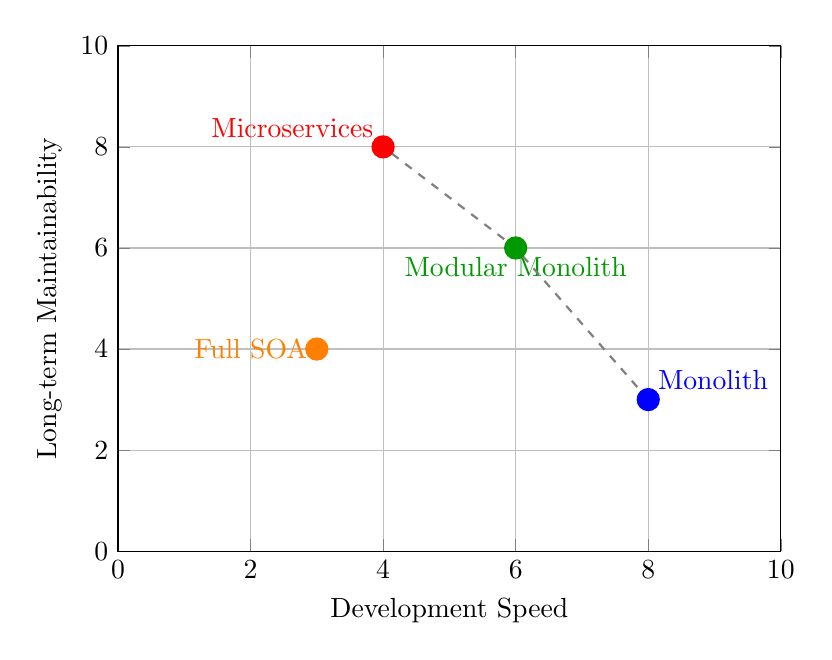
\begin{tikzpicture}
\begin{axis}[
    xlabel={Development Speed},
    ylabel={Long-term Maintainability},
    xmin=0, xmax=10,
    ymin=0, ymax=10,
    grid=major,
    width=10cm,
    height=8cm
]
    % Options
    \addplot[only marks, mark=*, mark size=4pt, blue] coordinates {(8,3)} node[anchor=south west] {Monolith};
    \addplot[only marks, mark=*, mark size=4pt, red] coordinates {(4,8)} node[anchor=south east] {Microservices};
    \addplot[only marks, mark=*, mark size=4pt, green!60!black] coordinates {(6,6)} node[anchor=north] {Modular Monolith};
    \addplot[only marks, mark=*, mark size=4pt, orange] coordinates {(3,4)} node[anchor=east] {Full SOA};
    
    % Pareto frontier
    \addplot[dashed, gray, thick] coordinates {(8,3) (6,6) (4,8)};
\end{axis}
\end{tikzpicture}
\caption{Architecture Style Tradeoff Visualization}
\end{figure}

%==============================================================================
\section{Architectural Patterns and Styles}
%==============================================================================

\subsection{Pattern Selection Rationale}

Architectural patterns encode proven solutions to recurring problems. Documenting why specific patterns were chosen connects the architecture to its design drivers.

\subsection{Pattern Documentation}

For each major pattern employed, document its selection rationale.

\begin{longtable}{@{}L{2.8cm} L{3.5cm} L{3.5cm} L{2.5cm}@{}}
\caption{Architectural Pattern Selection} \\
\toprule
\textbf{Pattern} & \textbf{Problem Addressed} & \textbf{Quality Attributes} & \textbf{ADR Reference} \\
\midrule
\endfirsthead
\toprule
\textbf{Pattern} & \textbf{Problem Addressed} & \textbf{Quality Attributes} & \textbf{ADR Reference} \\
\midrule
\endhead
\bottomrule
\endlastfoot
Microservices & Independent deployment; team autonomy & Modifiability; Scalability & ADR-007 \\
Event Sourcing & Audit trail; temporal queries & Auditability; Recoverability & ADR-009 \\
CQRS & Separate read/write optimization & Performance; Scalability & ADR-010 \\
API Gateway & Unified entry point; cross-cutting concerns & Security; Manageability & ADR-011 \\
Circuit Breaker & Cascading failure prevention & Availability; Resilience & ADR-012 \\
Saga & Distributed transaction coordination & Consistency; Resilience & ADR-013 \\
\end{longtable}

\subsection{Pattern Interaction Map}

\begin{figure}[H]
\centering
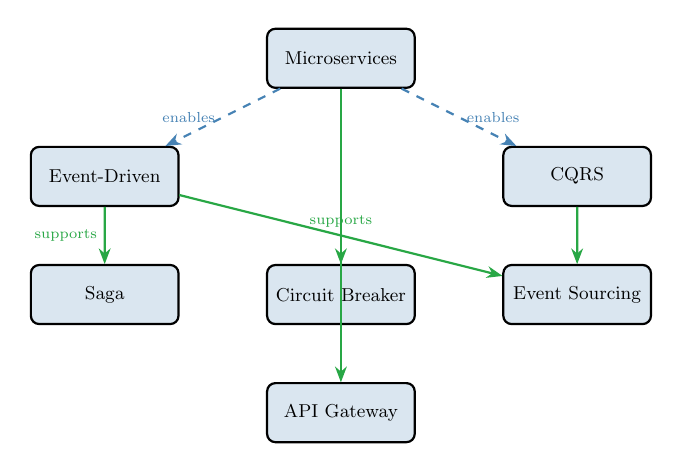
\begin{tikzpicture}[
    scale=0.75,
    transform shape,
    pattern/.style={draw, thick, fill=decisioncolor!20, minimum width=2.5cm, minimum height=1cm, rounded corners=3pt, font=\small},
    supports/.style={-{Stealth[length=2mm]}, thick, successgreen},
    enables/.style={-{Stealth[length=2mm]}, thick, decisioncolor, dashed}
]
    % Patterns
    \node[pattern] (micro) at (0,4) {Microservices};
    \node[pattern] (event) at (-4,2) {Event-Driven};
    \node[pattern] (cqrs) at (4,2) {CQRS};
    \node[pattern] (saga) at (-4,0) {Saga};
    \node[pattern] (es) at (4,0) {Event Sourcing};
    \node[pattern] (cb) at (0,0) {Circuit Breaker};
    \node[pattern] (gw) at (0,-2) {API Gateway};
    
    % Relationships
    \draw[enables] (micro) -- node[left, font=\scriptsize] {enables} (event);
    \draw[enables] (micro) -- node[right, font=\scriptsize] {enables} (cqrs);
    \draw[supports] (event) -- node[left, font=\scriptsize] {supports} (saga);
    \draw[supports] (event) -- node[above, font=\scriptsize] {supports} (es);
    \draw[supports] (cqrs) -- (es);
    \draw[supports] (micro) -- (cb);
    \draw[supports] (micro) -- (gw);
\end{tikzpicture}
\caption{Pattern Relationships in the Architecture}
\end{figure}

\subsection{Pattern Application Guidelines}

Document how patterns should be applied consistently across the system.

\begin{decisionbox}[Pattern: Circuit Breaker Application Guidelines]

\textbf{When to Apply:}
\begin{itemize}[nosep]
    \item All synchronous calls to external services
    \item All synchronous inter-service calls
    \item Database connections (with appropriate thresholds)
\end{itemize}

\textbf{Configuration Standards:}
\begin{itemize}[nosep]
    \item Failure threshold: 5 failures in 10 seconds
    \item Open duration: 30 seconds
    \item Half-open test requests: 3
    \item Timeout: Match SLA of downstream service
\end{itemize}

\textbf{Fallback Strategies:}
\begin{itemize}[nosep]
    \item Return cached data where acceptable
    \item Return degraded response with explanation
    \item Queue request for later retry
    \item Fail fast with clear error message
\end{itemize}

\textbf{Monitoring:}
\begin{itemize}[nosep]
    \item Alert when circuit opens
    \item Track circuit state transitions
    \item Dashboard for all circuit breaker states
\end{itemize}
\end{decisionbox}

%==============================================================================
\section{Risks and Technical Debt}
%==============================================================================

\subsection{Architectural Risk Management}

Architectural decisions involve uncertainty. Documenting risks ensures they are managed proactively rather than discovered in production.

\subsubsection{Risk Identification}

\begin{longtable}{@{}L{1cm} L{3cm} L{2cm} L{2cm} L{4.2cm}@{}}
\caption{Architectural Risk Register} \\
\toprule
\textbf{ID} & \textbf{Risk Description} & \textbf{Probability} & \textbf{Impact} & \textbf{Mitigation Strategy} \\
\midrule
\endfirsthead
\toprule
\textbf{ID} & \textbf{Risk Description} & \textbf{Probability} & \textbf{Impact} & \textbf{Mitigation Strategy} \\
\midrule
\endhead
\bottomrule
\endlastfoot
R-01 & Kafka cluster failure causes event loss & Low & Critical & Multi-AZ deployment; replication factor 3; disaster recovery runbook \\
R-02 & Database scaling limits reached before migration & Medium & High & Monitor growth; prepared sharding strategy; Aurora Serverless evaluation \\
R-03 & Team unable to maintain microservices complexity & Medium & High & Platform team support; standardization; training program \\
R-04 & Third-party payment provider outage & Medium & Critical & Secondary provider integration; graceful degradation \\
R-05 & Event schema evolution breaks consumers & High & Medium & Schema registry; compatibility rules; consumer contract testing \\
\end{longtable}

\subsubsection{Risk Heat Map}

\begin{figure}[H]
\centering
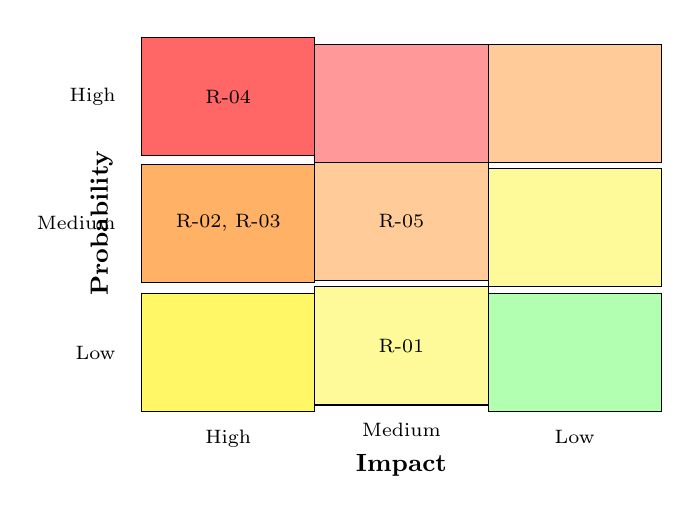
\begin{tikzpicture}[
    scale=0.9,
    cell/.style={minimum width=2.2cm, minimum height=1.5cm, draw, font=\scriptsize}
]
    % Grid
    \matrix (m) [matrix of nodes, nodes={cell}, column sep=-\pgflinewidth, row sep=-\pgflinewidth] {
        |[fill=red!60]| R-04 & |[fill=red!40]| & |[fill=orange!40]| \\
        |[fill=orange!60]| R-02, R-03 & |[fill=orange!40]| R-05 & |[fill=yellow!40]| \\
        |[fill=yellow!60]| & |[fill=yellow!40]| R-01 & |[fill=green!30]| \\
    };
    
    % Labels
    \node[left=0.5cm of m-2-1, font=\small\bfseries, rotate=90, anchor=center] {Probability};
    \node[below=0.5cm of m-3-2, font=\small\bfseries] {Impact};
    
    % Axis labels
    \node[left=0.2cm of m-1-1, font=\scriptsize] {High};
    \node[left=0.2cm of m-2-1, font=\scriptsize] {Medium};
    \node[left=0.2cm of m-3-1, font=\scriptsize] {Low};
    
    \node[below=0.1cm of m-3-1, font=\scriptsize] {High};
    \node[below=0.1cm of m-3-2, font=\scriptsize] {Medium};
    \node[below=0.1cm of m-3-3, font=\scriptsize] {Low};
\end{tikzpicture}
\caption{Risk Heat Map}
\end{figure}

\subsection{Technical Debt Documentation}

Technical debt is intentional deviation from ideal architecture, accepted for short-term benefit with planned future remediation.

\begin{definition}
\textbf{Technical Debt} is the implied cost of additional rework caused by choosing an easier solution now instead of using a better approach that would take longer. Like financial debt, it incurs ``interest'' in the form of increased maintenance cost and reduced agility.
\end{definition}

\subsubsection{Technical Debt Categories}

\begin{longtable}{@{}L{3cm} L{4.5cm} L{5cm}@{}}
\caption{Technical Debt Categories} \\
\toprule
\textbf{Category} & \textbf{Description} & \textbf{Examples} \\
\midrule
\endfirsthead
\toprule
\textbf{Category} & \textbf{Description} & \textbf{Examples} \\
\midrule
\endhead
\bottomrule
\endlastfoot
Deliberate/Prudent & Conscious choice with clear payoff & ``Ship now, refactor before scale'' \\
Deliberate/Reckless & Conscious choice ignoring consequences & ``No time for design'' \\
Inadvertent/Prudent & Learned better approach after building & ``Now we know how to do it properly'' \\
Inadvertent/Reckless & Due to lack of skill or knowledge & ``What's layering?'' \\
\end{longtable}

\subsubsection{Technical Debt Register}

\begin{longtable}{@{}L{1cm} L{3cm} L{2cm} L{2cm} L{4.2cm}@{}}
\caption{Technical Debt Register} \\
\toprule
\textbf{ID} & \textbf{Debt Description} & \textbf{Interest Cost} & \textbf{Payoff Effort} & \textbf{Remediation Plan} \\
\midrule
\endfirsthead
\toprule
\textbf{ID} & \textbf{Debt Description} & \textbf{Interest Cost} & \textbf{Payoff Effort} & \textbf{Remediation Plan} \\
\midrule
\endhead
\bottomrule
\endlastfoot
TD-01 & Monolithic user service (auth + profile + preferences) & Medium: harder to scale auth independently & 3 sprints & Split in Q3; extract auth service first \\
TD-02 & Hardcoded feature flags in code & High: deployments needed for flag changes & 1 sprint & Implement LaunchDarkly in Q2 \\
TD-03 & Synchronous inventory checks at checkout & Low: works at current scale & 2 sprints & Convert to async reservation when $>$5K orders/hour \\
TD-04 & No automated performance tests & Medium: manual testing delays releases & 2 sprints & Implement Gatling suite Q2 \\
TD-05 & Direct database access from API layer & High: tight coupling; hard to optimize & 4 sprints & Introduce repository pattern; scheduled for H2 \\
\end{longtable}

\subsection{Debt Repayment Strategy}

\begin{bestpractice}
\textbf{Managing Technical Debt:}

\textbf{Track It:} Maintain a technical debt register as part of the architecture documentation.

\textbf{Quantify It:} Estimate ``interest'' (ongoing cost) and ``principal'' (remediation cost) for prioritization.

\textbf{Budget for It:} Allocate capacity (e.g., 20\% of sprints) for debt repayment.

\textbf{Prevent It:} Use architecture reviews and coding standards to prevent inadvertent debt.

\textbf{Communicate It:} Ensure stakeholders understand the cost of carrying debt.

\textbf{Prioritize It:} Pay high-interest debt first; defer low-interest debt that may never need payment.
\end{bestpractice}

%==============================================================================
\section{Traceability}
%==============================================================================

\subsection{Importance of Traceability}

Traceability connects decisions to their drivers and consequences, enabling impact analysis when requirements change, validation that decisions satisfy requirements, compliance demonstration for audits, and knowledge navigation across documentation.

\subsection{Traceability Matrix}

\begin{longtable}{@{}L{1.5cm} L{3cm} L{3cm} L{2.5cm} L{2.2cm}@{}}
\caption{Decision Traceability Matrix} \\
\toprule
\textbf{Decision} & \textbf{Requirements} & \textbf{Quality Scenarios} & \textbf{Elements} & \textbf{Validation} \\
\midrule
\endfirsthead
\toprule
\textbf{Decision} & \textbf{Requirements} & \textbf{Quality Scenarios} & \textbf{Elements} & \textbf{Validation} \\
\midrule
\endhead
\bottomrule
\endlastfoot
ADR-001 & ASR-01, ASR-04 & QA-PERF-001, QA-REL-002 & ORDER-DB, INV-DB & Load test; backup test \\
ADR-002 & ASR-02, ASR-04 & QA-AVAIL-001, QA-AUDIT-001 & EVENT-BUS, all services & Chaos testing; replay test \\
ADR-003 & ASR-01, ASR-03 & QA-SCALE-001 & K8s cluster & Scale test; failover test \\
ADR-004 & CON-03 & QA-SEC-001 & AUTH-SVC & Penetration test; audit \\
\end{longtable}

\subsection{Bidirectional Tracing}

\subsubsection{Forward Tracing: Requirements to Decisions}

\begin{longtable}{@{}L{2cm} L{5.5cm} L{5cm}@{}}
\caption{Requirements to Decisions Tracing} \\
\toprule
\textbf{Requirement} & \textbf{Description} & \textbf{Satisfied By Decisions} \\
\midrule
\endfirsthead
\toprule
\textbf{Requirement} & \textbf{Description} & \textbf{Satisfied By Decisions} \\
\midrule
\endhead
\bottomrule
\endlastfoot
ASR-01 & Process 10,000 orders/minute at peak & ADR-001, ADR-002, ADR-003, ADR-010 \\
ASR-02 & Real-time inventory across 500 stores & ADR-002, ADR-009 \\
ASR-03 & Enable A/B testing of all features & ADR-003, ADR-014 \\
ASR-04 & Maintain audit trail for 7 years & ADR-001, ADR-002, ADR-009 \\
CON-03 & PCI-DSS Level 1 compliance & ADR-004, ADR-015, ADR-016 \\
\end{longtable}

\subsubsection{Backward Tracing: Decisions to Requirements}

\begin{longtable}{@{}L{1.5cm} L{4cm} L{7cm}@{}}
\caption{Decisions to Requirements Tracing} \\
\toprule
\textbf{Decision} & \textbf{Decision Summary} & \textbf{Driven By Requirements} \\
\midrule
\endfirsthead
\toprule
\textbf{Decision} & \textbf{Decision Summary} & \textbf{Driven By Requirements} \\
\midrule
\endhead
\bottomrule
\endlastfoot
ADR-001 & PostgreSQL for primary DB & ASR-01 (ACID for orders), ASR-04 (audit), CON-02 (team skills) \\
ADR-002 & Event-driven architecture & ASR-02 (real-time), ASR-04 (audit), QA-AVAIL-001 (resilience) \\
ADR-009 & Event sourcing for orders & ASR-04 (audit), ASR-02 (temporal queries), QA-AUDIT-001 \\
\end{longtable}

\subsection{Validation Coverage}

Track how decisions are validated to ensure they achieve intended outcomes.

\begin{longtable}{@{}L{1.5cm} L{3cm} L{3cm} L{2cm} L{2.5cm}@{}}
\caption{Decision Validation Coverage} \\
\toprule
\textbf{Decision} & \textbf{Validation Method} & \textbf{Validation Artifact} & \textbf{Frequency} & \textbf{Owner} \\
\midrule
\endfirsthead
\toprule
\textbf{Decision} & \textbf{Validation Method} & \textbf{Validation Artifact} & \textbf{Frequency} & \textbf{Owner} \\
\midrule
\endhead
\bottomrule
\endlastfoot
ADR-001 & Load testing & Gatling scripts; reports & Pre-release & QA Team \\
ADR-002 & Chaos engineering & Gremlin scenarios & Monthly & SRE Team \\
ADR-003 & Scale testing & K6 scripts; metrics & Quarterly & Platform Team \\
ADR-004 & Security audit & Pen test report & Annually & Security Team \\
ADR-009 & Event replay testing & Replay scripts; comparison & Pre-release & Dev Team \\
\end{longtable}

%==============================================================================
\section{Decision Governance}
%==============================================================================

\subsection{Decision-Making Process}

Establish a clear process for making and documenting architectural decisions.

\begin{figure}[H]
\centering
\begin{tikzpicture}[
    scale=0.75,
    transform shape,
    step/.style={draw, thick, fill=decisioncolor!20, minimum width=2.5cm, minimum height=1cm, rounded corners=3pt, font=\small},
    arrow/.style={-{Stealth[length=2.5mm]}, thick}
]
    % Steps
    \node[step] (identify) at (0,0) {1. Identify Need};
    \node[step] (research) at (4,0) {2. Research Options};
    \node[step] (evaluate) at (8,0) {3. Evaluate Alternatives};
    \node[step] (propose) at (0,-2.5) {4. Propose Decision};
    \node[step] (review) at (4,-2.5) {5. Review \& Discuss};
    \node[step] (decide) at (8,-2.5) {6. Decide};
    \node[step] (document) at (2,-5) {7. Document ADR};
    \node[step] (implement) at (6,-5) {8. Implement};
    
    % Arrows
    \draw[arrow] (identify) -- (research);
    \draw[arrow] (research) -- (evaluate);
    \draw[arrow] (evaluate) -- (propose);
    \draw[arrow] (propose) -- (review);
    \draw[arrow] (review) -- (decide);
    \draw[arrow] (decide) -- (document);
    \draw[arrow] (document) -- (implement);
    
    % Feedback loop
    \draw[arrow, dashed] (review) to[bend left=30] node[above, font=\scriptsize] {revise} (propose);
\end{tikzpicture}
\caption{Decision-Making Process}
\end{figure}

\subsection{Decision Authority Matrix}

Define who has authority to make different types of decisions.

\begin{longtable}{@{}L{4cm} L{3cm} L{2.5cm} L{3cm}@{}}
\caption{Decision Authority Matrix (RACI)} \\
\toprule
\textbf{Decision Type} & \textbf{Responsible} & \textbf{Accountable} & \textbf{Consulted} \\
\midrule
\endfirsthead
\toprule
\textbf{Decision Type} & \textbf{Responsible} & \textbf{Accountable} & \textbf{Consulted} \\
\midrule
\endhead
\bottomrule
\endlastfoot
Strategic (patterns, platforms) & Architecture Team & Chief Architect & Tech Leads; CTO \\
Tactical (service design) & Tech Lead & Chief Architect & Architecture Team \\
Implementation (libraries, tools) & Developer & Tech Lead & Team \\
Cross-cutting (security, compliance) & Specialist & Chief Architect & Legal; Security \\
Emergency (production fixes) & On-call Engineer & Tech Lead & Architecture Team \\
\end{longtable}

\subsection{Review Cadence}

\begin{longtable}{@{}L{3cm} L{3cm} L{3.5cm} L{3cm}@{}}
\caption{Decision Review Schedule} \\
\toprule
\textbf{Review Type} & \textbf{Frequency} & \textbf{Scope} & \textbf{Participants} \\
\midrule
\endfirsthead
\toprule
\textbf{Review Type} & \textbf{Frequency} & \textbf{Scope} & \textbf{Participants} \\
\midrule
\endhead
\bottomrule
\endlastfoot
ADR Review & Per ADR (async + meeting if needed) & Single decision & Author + reviewers \\
Architecture Sync & Weekly & Current decisions; blockers & Architecture Team \\
Architecture Review Board & Monthly & Strategic decisions & Architects + leads \\
Technical Debt Review & Quarterly & Debt register; priorities & Tech leads + PMs \\
Architecture Retrospective & Semi-annually & All decisions; lessons learned & Full team \\
\end{longtable}

%==============================================================================
\section{Open Issues and Future Decisions}
%==============================================================================

\subsection{Pending Decisions}

Document decisions that are needed but not yet made.

\begin{longtable}{@{}L{1.2cm} L{3.5cm} L{2cm} L{2.5cm} L{3cm}@{}}
\caption{Pending Decision Queue} \\
\toprule
\textbf{ID} & \textbf{Decision Needed} & \textbf{Urgency} & \textbf{Target Date} & \textbf{Blocker/Dependencies} \\
\midrule
\endfirsthead
\toprule
\textbf{ID} & \textbf{Decision Needed} & \textbf{Urgency} & \textbf{Target Date} & \textbf{Blocker/Dependencies} \\
\midrule
\endhead
\bottomrule
\endlastfoot
PD-01 & GraphQL vs REST for mobile API & High & 2024-03-01 & Mobile team input needed \\
PD-02 & Multi-region deployment strategy & Medium & 2024-04-15 & Cost analysis pending \\
PD-03 & Search engine selection & Medium & 2024-03-15 & Requirements clarification \\
PD-04 & Observability platform selection & Low & 2024-05-01 & Budget approval \\
\end{longtable}

\subsection{Questions and Unknowns}

\begin{longtable}{@{}L{1cm} L{5cm} L{3cm} L{3.5cm}@{}}
\caption{Open Questions} \\
\toprule
\textbf{ID} & \textbf{Question} & \textbf{Impact If Unresolved} & \textbf{Owner / Due Date} \\
\midrule
\endfirsthead
\toprule
\textbf{ID} & \textbf{Question} & \textbf{Impact If Unresolved} & \textbf{Owner / Due Date} \\
\midrule
\endhead
\bottomrule
\endlastfoot
Q-01 & What is the expected international expansion timeline? & Multi-region decision depends on this & Product / Feb 15 \\
Q-02 & Will we need to support on-premise deployment? & Affects containerization strategy & Sales / March 1 \\
Q-03 & What are the actual peak traffic projections for Year 2? & Influences scaling architecture & Analytics / Feb 28 \\
Q-04 & Are there planned acquisitions that would require integration? & May affect integration architecture & Exec / Ongoing \\
\end{longtable}

%==============================================================================
\section{Appendix A: ADR Template}
%==============================================================================

\begin{tcolorbox}[colback=white, colframe=flowcolor, title=\textbf{Architecture Decision Record Template}]

\textbf{ADR-NNN: [Short Title]}

\vspace{0.3cm}
\textbf{Status:} [Proposed | Accepted | Deprecated | Superseded by ADR-XXX]

\textbf{Date:} YYYY-MM-DD

\textbf{Deciders:} [List of people involved in decision]

\vspace{0.3cm}
\textbf{Context}

[Describe the issue motivating this decision. What is the problem? What are the constraints? What forces are at play?]

\vspace{0.3cm}
\textbf{Decision}

[State the decision. Use active voice: ``We will...'']

\vspace{0.3cm}
\textbf{Consequences}

[What are the results of this decision? Include both positive and negative consequences.]

\textit{Positive:}
\begin{itemize}[nosep]
    \item [Benefit 1]
    \item [Benefit 2]
\end{itemize}

\textit{Negative:}
\begin{itemize}[nosep]
    \item [Drawback 1]
    \item [Drawback 2]
\end{itemize}

\textit{Risks:}
\begin{itemize}[nosep]
    \item [Risk 1]
\end{itemize}

\vspace{0.3cm}
\textbf{Alternatives Considered}

[What other options were evaluated?]

\textbf{Alternative 1:} [Description and why rejected]

\textbf{Alternative 2:} [Description and why rejected]

\vspace{0.3cm}
\textbf{Related Decisions}

[Links to related ADRs]

\vspace{0.3cm}
\textbf{References}

[Links to relevant documentation, research, or resources]
\end{tcolorbox}

%==============================================================================
\section{Appendix B: Decision Checklist}
%==============================================================================

\subsection{Before Making a Decision}

\begin{itemize}[leftmargin=2cm]
    \item[$\square$] Problem is clearly understood and documented
    \item[$\square$] Relevant stakeholders are identified
    \item[$\square$] Design drivers (QAs, constraints, requirements) are documented
    \item[$\square$] Multiple alternatives have been identified
    \item[$\square$] Evaluation criteria are defined and weighted
    \item[$\square$] Alternatives have been systematically evaluated
    \item[$\square$] Tradeoffs are understood and documented
    \item[$\square$] Risks are identified
\end{itemize}

\subsection{When Documenting a Decision}

\begin{itemize}[leftmargin=2cm]
    \item[$\square$] Context explains the situation objectively
    \item[$\square$] Decision is stated clearly and actionably
    \item[$\square$] Both positive and negative consequences are listed
    \item[$\square$] Rejected alternatives and reasons are documented
    \item[$\square$] Traceability to requirements is established
    \item[$\square$] Validation approach is identified
    \item[$\square$] ADR is reviewed by appropriate stakeholders
    \item[$\square$] ADR is stored in version control
\end{itemize}

\subsection{After Making a Decision}

\begin{itemize}[leftmargin=2cm]
    \item[$\square$] Decision is communicated to affected teams
    \item[$\square$] Implementation guidance is provided if needed
    \item[$\square$] Validation tests are implemented
    \item[$\square$] Metrics/monitoring for consequences are established
    \item[$\square$] Technical debt register is updated if applicable
    \item[$\square$] Decision log summary is updated
\end{itemize}

%==============================================================================
\section{Appendix C: Glossary}
%==============================================================================

\begin{description}[leftmargin=3cm, style=nextline]
    \item[ADR] Architecture Decision Record; a document capturing a single architectural decision
    \item[ASR] Architecturally Significant Requirement; a requirement with significant impact on architecture
    \item[ATAM] Architecture Tradeoff Analysis Method; a structured approach to evaluating architecture quality
    \item[Design Driver] A force (requirement, constraint, goal) that shapes architectural decisions
    \item[Quality Attribute] A measurable property of a system such as performance, security, or availability
    \item[Quality Attribute Scenario] A concrete, testable specification of a quality attribute requirement
    \item[Rationale] The reasoning behind a decision, including alternatives considered and tradeoffs made
    \item[Technical Debt] Implied cost of future rework caused by choosing easier solutions now
    \item[Traceability] The ability to relate decisions to requirements and other artifacts
    \item[Tradeoff] A situation where improving one quality attribute negatively impacts another
\end{description}

%==============================================================================
\section{Appendix D: References}
%==============================================================================

\begin{enumerate}
    \item Nygard, M. (2011). ``Documenting Architecture Decisions.'' Cognitect Blog. Retrieved from \url{https://cognitect.com/blog/2011/11/15/documenting-architecture-decisions}
    
    \item Clements, P., et al. (2010). \textit{Documenting Software Architectures: Views and Beyond} (2nd ed.). Addison-Wesley.
    
    \item Bass, L., Clements, P., \& Kazman, R. (2021). \textit{Software Architecture in Practice} (4th ed.). Addison-Wesley.
    
    \item Keeling, M. (2017). \textit{Design It! From Programmer to Software Architect}. Pragmatic Bookshelf.
    
    \item Kazman, R., Klein, M., \& Clements, P. (2000). ``ATAM: Method for Architecture Evaluation.'' SEI Technical Report CMU/SEI-2000-TR-004.
    
    \item Tyree, J., \& Akerman, A. (2005). ``Architecture Decisions: Demystifying Architecture.'' IEEE Software, 22(2), 19-27.
    
    \item Cunningham, W. (1992). ``The WyCash Portfolio Management System.'' OOPSLA '92 Experience Report. (Origin of ``technical debt'' metaphor)
    
    \item IEEE. (2011). \textit{ISO/IEC/IEEE 42010:2011 Systems and Software Engineering---Architecture Description}.
\end{enumerate}

\end{document}